\documentclass{article}

\usepackage[letterpaper,portrait,margin=1in]{geometry}

\usepackage{amsmath, amsfonts, amsthm, amssymb}
\usepackage{graphicx, float}
\usepackage{mathtools}
\usepackage{siunitx}
\usepackage{titlesec}
\usepackage{interval}
\usepackage{titling}
\usepackage{multicol}

\intervalconfig {
	soft open fences
}

\usepackage{tikz}
\usetikzlibrary{positioning}
\usetikzlibrary{angles,quotes}

\newtheorem*{theorem*}{Theorem}

%opening
\title{Problem Set \#33, Part 2}
\author{Jayden Li}
\date{December 8, 2023}

\begin{document}

\newgeometry{top=0.4in,bottom=1in,right=1in,left=1in}

\linespread{1.25}
\fontsize{12pt}{12pt}\selectfont

\maketitle

\begin{multicols}{2}

\section*{Problem 2}
	\begin{itemize}
	\item[(b)]
	\begin{proof}
		$\begin{aligned}[t]
			&\lim\limits_{h\to0}\frac{\cos\left(h\right)-1}{h} \\
			=&\lim\limits_{h\to0}\frac{\cos\left(2\cdot\frac{h}{h}\right)-1}{2} \\
			=&\lim\limits_{h\to0}\frac{2\cos^2h-1-1}{h} \\
			=&2\lim\limits_{h\to0}\frac{\cos^2h-1}{h} \\
			=&2\lim\limits_{h\to0}\frac{-\sin^2h}{h} \\
			=&2\lim\limits_{h\to0}\left(\frac{-\sin h}{h}\cdot\sin h\right) \\
			=&-2\sin\left(0\right)\cdot\lim\limits_{h\to0}\frac{\sin h}{h} \\
			=&-2\cdot0\cdot1 \\
			=&\boxed{0}
		\end{aligned} \\$
	\end{proof}
\end{itemize}
\section*{Problem 3}
\begin{itemize}
	\item[(a)]
	$\begin{aligned}[t]
		&\lim\limits_{h\to\infty}\frac{\sin h}{h}=0 \\
		&\lim\limits_{h\to-\infty}\frac{\sin h}{h}=0 \\
	\end{aligned}$
	\flushleft{
	In both limits, $\sin h$ stays between $-1$ and $1$. As $h\to\infty$,
	the quotient of a number between $-1$ and $1$ approaches 0. Even
	though $\sin h$ is alternating, the quotient still approaches 0
	as the denonimator grows.}

	\item[(b)]
	$\begin{aligned}[t]
		f\left(x\right)&=\frac{\sin x}{x} \\
		\frac{\sin x}{x}&=0 \\
		\sin x&=0,\,x\neq0 \\
		\Aboxed{x&=\pi n,\,x\neq0,\,n\in\mathbb{Z}} \\
		x&=\hdots,\,-2\pi,\,-\pi,\,\pi,\,2\pi,\,\hdots \\
	\end{aligned}$
\end{itemize}
\end{multicols}

\begin{figure}[h]
	\centering
	\includegraphics[width=\textwidth]{ps34q3b.png}
\end{figure}

\pagebreak
\title{Problem Set \#34}
\maketitle

\section*{Problem 5}
\begin{itemize}
	\item[(a)]
		True. The domain of $\arcsin y$ is $-1\leq y\leq1$, and
		by the definition of the $\arcsin y$ as the inverse of
		$\sin y$, $\sin\left(\arcsin y\right)$ must equal $y$
		inside the domain of $\arcsin y$.
	\item[(b)]
		False. $\arcsin\left(\sin5\pi\right)=\arcsin0=0$,
		$0\neq5\pi$.
	\item[(c)]
		False. $\arccos\left(\cos5\pi\right)=\arccos\left(-1\right)
		=\pi$, $\pi\neq5\pi$.
	\item[(d)]
		True. $\cos\left(\arccos y\right)=y$ within the domain of
		$\arccos y$, and $-1\leq y\leq1$ is the domain of $\arccos y$.
	\item[(e)]
		True.
		\begin{proof}
		\leavevmode\vspace*{-\baselineskip}
			\begin{align*}
				\text{Let }y&=\arcsin x \\
			\sin y&=\sin\left(\arcsin x\right),\,
			-\frac{\pi}{2}\leq y\leq\frac{\pi}{2},
			\text{ as}-\frac{\pi}{2}\leq\arcsin x\leq\frac{\pi}{2} \\
			\sin y&=x,\,-\frac{\pi}{2}\leq y\leq\frac{\pi}{2} \\
			-\sin y&=-x,\,-\frac{\pi}{2}\leq y\leq\frac{\pi}{2} \\
			\sin\left(-y\right)&=-x,\,-\frac{\pi}{2}\leq y\leq\frac{\pi}{2} \\
			\arcsin\left(\sin\left(-y\right)\right)&=\arcsin\left(-x\right),\,
			-\frac{\pi}{2}\leq y\leq\frac{\pi}{2} \\
			-y&=\arcsin\left(-x\right) \\
			\arcsin x&=-\arcsin\left(-x\right) \\
		\end{align*}
		\end{proof} 
	\item[(f)]
		False. $\arccos\left(-1\right)=\pi$, $\arccos\left(1\right)=0$, $\pi\neq0$.
\end{itemize}

\pagebreak

\newgeometry{margin=1in}

\section*{Problem 8}
\begin{itemize}
	\item[(e)]
	\begin{align*}
		y=\arccos\left(\frac{x-3}{2x-1}\right)
	\end{align*}
	\begin{minipage}[t]{.45\textwidth}
	\begin{align*}
		\frac{x-3}{2x-1}&\geq-1 \\
		\frac{x-3}{2x-1}+\frac{2x-1}{2x-1}&\geq0 \\
		\frac{3x-4}{2x-1}&\geq0 \\
		\\
		2x-1&=0 \\
		x&=\frac{1}{2} \\
		\\
		3x-4&=0 \\
		x&=\frac{4}{3} \\
	\end{align*}
	\centering
	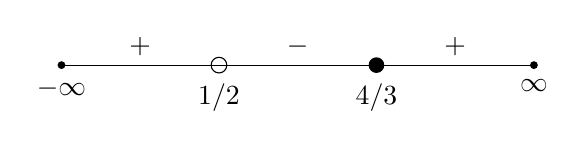
\begin{tikzpicture}	
		\draw
		(0,0) node[circle,fill,inner sep=1pt,label=below:$-\infty$](a){}
	 -- (2,0) node[circle,draw,inner sep=2pt,label=below:$1/2$](b){} node[midway,above]{$+$}
	 -- (4,0) node[circle,fill,inner sep=2pt,label=below:$4/3$](c){}node[midway,above]{$-$}
	 -- (6,0) node[circle,fill,inner sep=1pt,label=below:$\infty$](d){} node[midway,above]{$+$};
	\end{tikzpicture}
	\[
		x\in
		\interval[scaled,open left,open right]{-\infty}{\frac{1}{2}}\cup
		\interval[scaled,open right]{\frac{4}{3}}{\infty}
	\]
	\end{minipage}
	\begin{minipage}[t]{.45\textwidth}
	\begin{align*}
		\frac{x-3}{2x-1}&\leq1 \\
		\frac{x-3}{2x-1}-\frac{2x-1}{2x-1}&\leq0 \\
		\frac{-x-2}{2x-1}&\leq0 \\
		\\
		2x-1&=0 \\
		x&=\frac{1}{2} \\
		\\
		-x-2&=0 \\
		x&=-2 \\
	\end{align*}
	\centering
	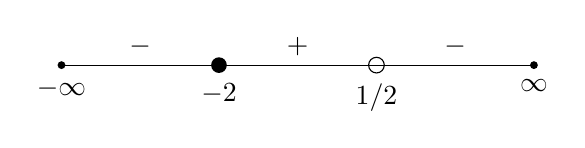
\begin{tikzpicture}	
		\draw
		(0,0) node[circle,fill,inner sep=1pt,label=below:$-\infty$](a){}
	 -- (2,0) node[circle,fill,inner sep=2pt,label=below:$-2$](b){} node[midway,above]{$-$}
	 -- (4,0) node[circle,draw,inner sep=2pt,label=below:$1/2$](c){} node[midway,above]{$+$}
	 -- (6,0) node[circle,fill,inner sep=1pt,label=below:$\infty$](d){} node[midway,above]{$-$};
	\end{tikzpicture}
	\[
		x\in
		\interval[scaled,open left]{-\infty}{-2}\cup
		\interval[scaled,open left,open right]{\frac{1}{2}}{\infty}
	\] \\
	\end{minipage}
	\begin{gather*}
		\\
		x\in
		\left(\interval[scaled,open left,open right]{-\infty}{\frac{1}{2}}\cup
		\interval[scaled,open right]{\frac{4}{3}}{\infty}\right)
		\cap\left(\interval[scaled,open left]{-\infty}{-2}\cup
		\interval[scaled,open left,open right]{\frac{1}{2}}{\infty}\right) \\
		\boxed{x\in
		\interval[scaled,open left]{-\infty}{-2}\cup
		\interval[scaled,open right]{\frac{4}{3}}{\infty}} \\
	\end{gather*}
\end{itemize}

\pagebreak

\newgeometry{top=0.75in,bottom=1in,right=0.5in,left=0.5in}

\section*{Problem 9}
\begin{theorem*}$
	\arcsin x-\arcsin y=
	\arcsin\left(x\sqrt{1-y^2}-y\sqrt{1-x^2}\right)
$\end{theorem*}
	
\begin{proof}
	\begin{center}
	\begin{minipage}[t]{.45\textwidth}
	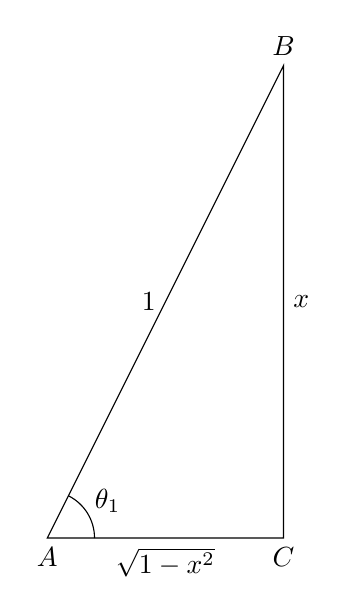
\begin{tikzpicture}[
		baseline=(current bounding box.north),
		ang/.style={draw, angle eccentricity=1.5,angle radius=0.6cm}
	]	
		\draw 
		(0,0) coordinate[label=below:{$A$}](A)
	 -- (3,0) coordinate[label=below:{$C$}](C) node[midway,below]{$\sqrt{1-x^2}$}
	 -- (3,6) coordinate[label=above:{$B$}](B) node[midway,right]{$x$}
	 -- cycle node[midway,above,left]{$1$}
	 	pic["$\theta_1$",ang]{angle=C--A--B};
	\end{tikzpicture}
	$\begin{aligned}[t]
		\\
		\text{Let }\theta_1&=\arcsin x \\
		\sin\theta_1&=\sin\left(\arcsin x\right) \\
		\frac{\text{opp}}{\text{hyp}}&=x \\
		\frac{BC}{AB}&=x \\
		\text{Let }BC&=x,\,AB=1 \\
		AC&=\sqrt{1-x^2} \\
		\\
		\sin\theta_1&=x \\
		\cos\theta_1&=\sqrt{1-x^2} \\
	\end{aligned}$
	\end{minipage}
	\begin{minipage}[t]{.45\textwidth}
	\begin{tikzpicture}[
		baseline=(current bounding box.north),
		ang/.style={draw, angle eccentricity=1.5,angle radius=0.6cm}
	]	
		\draw 
		(0,0) coordinate[label=below:{$D$}](D)
	 -- (3,0) coordinate[label=below:{$F$}](F) node[midway,below]{$\sqrt{1-y^2}$}
	 -- (3,6) coordinate[label=above:{$E$}](E) node[midway,right]{$y$}
	 -- cycle node[midway,above,left]{$1$}
	 	pic["$\theta_2$",ang]{angle=C--A--B};
	\end{tikzpicture}
	$\begin{aligned}[t]
		\\
		\text{Let }\theta_2&=\arcsin y \\
		\sin\theta_2&=\sin\left(\arcsin y\right) \\
		\frac{\text{opp}}{\text{hyp}}&=y \\
		\frac{EF}{DE}&=y \\
		\text{Let }EF&=y,\,DE=1 \\
		DF&=\sqrt{1-y^2} \\
		\\
		\sin\theta_2&=y \\
		\cos\theta_2&=\sqrt{1-y^2} \\
	\end{aligned}$
	\end{minipage}
	\end{center}

	\begin{align*}
		\text{RHS: }&\arcsin\left(x\sqrt{1-y^2}-y\sqrt{1-x^2}\right) \\
		&=\arcsin\left(\sin\theta_1\cos\theta_2-\sin\theta_2\cos\theta_1\right) \\
		&=\arcsin\left(\sin\left(\theta_1-\theta_2\right)\right) \\
		&=\theta_1-\theta_2\ \\
		&=\arcsin x-\arcsin y
	\end{align*}
\end{proof}

\pagebreak

\section*{Problem 10}
\begin{multicols}{2}
\begin{itemize}
	\item[(a)]
	\phantom{}
	\begin{figure}[H]
		\includegraphics[height=0.5\textheight]{ps34q10a.png}
	\end{figure}

	\item[(b)]
	\begin{flushleft}	
	$\arccos\left(\cos x\right)$ is periodic with period $2\pi$.
	This means that the graph on $\interval[scaled]{-\pi}{\pi}$
	repeats. Because $\arccos x$ is defined as the invrse of
	$\cos x$ on $\interval[scaled]{0}{\pi}$, $\arccos\left(
	\cos x\right)=x$.
	
	Let $\theta\in\interval[scaled]{-\pi}{0}$ and
	$\varphi=\theta+\pi$, so $\varphi\in\interval[scaled]
	{0}{\pi}$ and $\theta=\pi-\varphi$. $\arccos\left(\cos\left(
	\pi-\varphi\right)\right)=\arccos\left(\cos\theta\right)$. By
	angle addition identites, $\arccos\left(-\cos\varphi\right)=
	\arccos\left(\cos\theta\right)$. Now, we will prove that
	$\arccos\left(-\cos\varphi\right)=\pi-\varphi$.
	\end{flushleft}
	\begin{proof}
		\begin{gather*}
			-\cos\varphi=-\cos\varphi \\
			-\cos\varphi=\cos\pi\cos\varphi+\sin\pi\sin\varphi \\
			\cos\left(\arccos\left(-\cos\varphi\right)\right)
			=\cos\left(\pi-\varphi\right) \\
			\text{(This is fine because
			$\varphi$, $\pi-\varphi\in\interval[scaled]{0}{2\pi}$)} \\
			\arccos\left(-\cos\varphi\right)=\pi-\varphi
		\end{gather*}
	\end{proof}
	\begin{flushleft}
	From this identity, $\pi-\varphi=\arccos\left(\cos\theta
	\right)$. Substituting $\varphi=\theta+\pi$ gives $-\theta=
	\arccos\left(\cos\theta\right)$. Now, changing variable
	$\theta$ to $x$, we see that $y=-x$ on $\interval[scaled]
	{-\pi}{0}$.
	\end{flushleft}
\end{itemize}
\end{multicols}

\begin{figure}[H]
	\centering
	\includegraphics[height=0.3\textheight]{ps34q10b.png}
\end{figure}

\end{document}
